\documentclass[12pt]{article}
\usepackage[margin=1in]{geometry}
\usepackage{setspace}
\doublespacing
\usepackage[utf8]{inputenc}
\usepackage[T1]{fontenc}
\usepackage{times}
\usepackage{graphicx}
\usepackage{booktabs}
\usepackage{amsmath}
\usepackage{natbib}
\bibliographystyle{chicago}
\usepackage{hyperref}
\hypersetup{colorlinks=true,linkcolor=blue,citecolor=blue,urlcolor=blue}
\usepackage{caption}
\captionsetup{font=small,labelfont=bf}

\title{Two Javas:\\Spatial Segregation of Sacred and Administrative Landscapes\\in Volcanic Java and Its Consequences for Archaeological Inference}

\author{[Author removed for double-blind review]}

\date{}

\begin{document}
\maketitle

\begin{abstract}
The archaeological record of Java is commonly treated as uniformly sparse before 400~CE.
This paper demonstrates that the record is spatially structured along volcanic distance gradients.
Analysis of 142 temples (candi), 176 geocoded inscriptions, and 391 archaeological sites reveals two distinct archaeological worlds.
``Volcano Java'' (0--15~km from active volcanoes) is dominated by sacred architecture with relatively indigenous vocabulary, progressively buried at 2.4--6.2~mm/year.
``Court Java'' (15--30~km) is dominated by administrative inscriptions with Sanskrit-heavy content.
Candi peak at a median distance of 14.6~km from the nearest volcano; inscriptions peak at 27.6~km ($p < 0.000001$).
The temporal trend of increasing pre-Indic vocabulary ($\rho = 0.781$, $p < 0.0001$) occurs exclusively in the court zone.
After the 929~CE Mataram collapse, epigraphic activity abandons the court zone entirely, shifting to the periphery with indigenous-rich content.
Indigenous vocabulary correlates with burial depth ($\rho = 0.456$, $p < 0.0001$, controlling for inscription length), meaning that volcanic burial preferentially conceals the most culturally indigenous inscriptions.
Inscription counts cannot serve as proxies for population density without accounting for this spatial bias.
The textual record of ``Indianization'' was a 15-kilometre-wide court phenomenon, not a civilisation-wide transformation.
\end{abstract}

\noindent\textbf{Keywords:} spatial archaeology, volcanic taphonomy, Indianization, Old Javanese epigraphy, candi distribution, court zone, two Javas, archaeological bias


\section{Introduction}

Indonesian archaeology operates under an implicit assumption of uniform darkness: the record before 400~CE is sparse everywhere, and the Hindu-Buddhist period (5th--15th centuries) represents a civilisation-wide transformation.
This paper challenges both assumptions by showing that Java's archaeological record has a \emph{spatial structure} that correlates with volcanic geography.

The assumption of uniformity has deep roots.
When Coed\`{e}s compiled his synthesis of ``The Indianized States of Southeast Asia,'' he treated inscriptional evidence as representative of entire polities \citep{Coedes1968}.
Subsequent scholarship has refined his conclusions but retained the fundamental premise: that the visibility or absence of inscriptions reflects the presence or absence of complex society.
The regions of Java where inscriptions are abundant -- the Prambanan plain, the Solo valley, the Brantas basin -- are treated as centres of civilisation; the regions where inscriptions are scarce are treated as peripheries or hinterlands.

This premise is undermined by a simple geographic observation: sacred architecture (candi) and administrative inscriptions do not occupy the same space.
Candi cluster on volcanic slopes within 15~km of active craters, while inscriptions cluster 15--30~km away on the fertile plains where royal courts were established.
The median gap between these two archaeological populations -- 13 kilometres -- represents not a gradual transition but a fundamental division between two modes of cultural production: one physical and relatively indigenous, the other textual and heavily Sanskritized.

This spatial division has consequences for how we interpret the archaeological record.
If inscriptions are concentrated in the ``court zone'' (15--30~km from volcanoes) and this zone was the epicentre of Indianization, then using inscription counts as proxies for population density or cultural activity systematically overrepresents the Sanskritized court world and underrepresents the indigenous volcanic world.
The problem is compounded by taphonomy: volcanic sedimentation at 2.4--6.2~mm/year progressively buries the archaeological evidence of Volcano Java, while Court Java's stone inscriptions remain on or near the surface.

The 929~CE Mataram collapse provides a before-after observation that illuminates this spatial structure.
When the court system collapsed and the political centre shifted from Central to East Java, epigraphic activity migrated from the court zone to the periphery ($>$30~km), and the vocabulary shifted from Sanskrit-dominant to indigenous-rich \citep{Christie2001}.
This reveals that the indigenous substrate had been present all along, merely invisible in the court zone's inscriptional genre.
The Sanskrit overlay was removed, and the underlying indigenous cultural landscape became visible again.

We present five mutually reinforcing analyses drawn from a suite of 175 computational experiments:
\begin{enumerate}
    \item Spatial segregation of candi and inscriptions by volcanic distance (E104)
    \item Monotonic increase in site density with elevation (E100)
    \item Indigenous vocabulary scaling with burial depth, controlling for inscription length (E102)
    \item The court zone as the exclusive locus of pre-Indic vocabulary recovery (E103)
    \item Post-929~CE geographic relocation of epigraphic activity (E105)
\end{enumerate}

Together, these analyses constitute a \emph{spatial model of archaeological bias} that replaces the assumption of uniform darkness with a structured geography of differential visibility (Table~\ref{tab:summary}).

\begin{table}[htbp]
\centering
\caption{Summary of five analyses supporting the Two Javas model.}
\label{tab:summary}
\begin{tabular}{llll}
\toprule
\textbf{Analysis} & \textbf{Key statistic} & \textbf{$p$-value} & \textbf{Implication} \\
\midrule
Spatial segregation & Median gap = 13~km & $< 0.000001$ & Candi \& inscriptions \\
(E104) & MW $U = 8081$ & & occupy different zones \\
\addlinespace
Elevation gradient & Density 1.96 $\rightarrow$ 18.61 & $< 0.000001$ & Mountain sites = \\
(E100) & 9.5$\times$ increase & & buried population tip \\
\addlinespace
Vocab $\times$ depth & $\rho = 0.456$ (partial) & $< 0.0001$ & Burial hides \\
(E102) & 5.8$\times$ jump & & indigenous content \\
\addlinespace
Court zone trend & $\rho = 0.781$ & $< 0.0001$ & Indianization is \\
(E103) & (court only) & & zone-specific \\
\addlinespace
Post-929 relocation & 91\% Sanskrit $\rightarrow$ & -- & Collapse removes \\
(E105) & 89\% indigenous & & Sanskrit overlay \\
\bottomrule
\end{tabular}
\end{table}


\section{Background}

\subsection{Volcanic geography of Java}

Java lies on the Sunda Arc, where the Indo-Australian plate subducts beneath the Eurasian plate, producing one of the densest concentrations of active volcanoes on Earth.
The island hosts 45 active volcanoes \citep{GVP2024}, of which approximately 10 have been responsible for the majority of Holocene eruptions affecting the cultural heartland: Merapi, Kelud, Arjuno, Semeru, Bromo, Penanggungan, Lawu, Merbabu, Sindoro, and Sumbing.
These volcanoes have erupted repeatedly throughout the historical period.
Merapi alone has produced more than 60 eruptions in the last millennium \citep{Newhall2000, Gertisser2012}.

The archaeological consequence of this volcanism is progressive burial.
Lahars, pyroclastic density currents, and tephra fallout deposit material at rates of 2.4--6.2~mm/year on proximal slopes \citep{Lavigne2000}, accumulating metres of overburden over centuries.
The temples of Sambisari (6.5~m), Kimpulan (2.5~m), and Liyangan (6~m) demonstrate that significant Hindu-Buddhist structures can be buried completely within 500--1000 years of abandonment \citep{Putra2019, Abbas2016}.
Van Bemmelen's geological surveys documented burial of cultural surfaces throughout Central and East Java \citep{VanBemmelen1949}.

\subsection{The inscriptional record}

Java's pre-modern inscriptional corpus consists of approximately 268 stone and copper-plate inscriptions in the DHARMA EpiDoc archive \citep{DHARMA2024}, spanning the 5th to 15th centuries CE.
These inscriptions are overwhelmingly administrative in character: land grants (\textit{sima} charters), tax exemptions, and royal genealogies, composed in Sanskrit, Old Javanese, or a mixture of both.

The corpus is not randomly distributed.
As de Casparis noted, inscriptions cluster in areas associated with court activity -- the Kedu, Prambanan, and Brantas plains -- while the volcanic highlands and coastal lowlands are comparatively inscription-free \citep{Casparis1975}.
This clustering has traditionally been interpreted as reflecting the distribution of political power.
However, it may equally reflect the distribution of a particular \emph{genre} of evidence: administrative texts produced by and for court institutions.

\subsection{Candi distribution}

The term \textit{candi} refers to Hindu-Buddhist temple structures, of which 142 with reliable coordinates are known from archaeological inventories.
De Groot's spatial analysis of Central Javanese candi demonstrated that temples were oriented toward and clustered near major volcanoes, particularly Merapi and Penanggungan \citep{Degroot2009}.
This volcanic orientation is not coincidental: mountains are sacred in Javanese cosmology, identified with the cosmic Mount Meru and serving as abodes of ancestors \citep{Dumarcay1986, Kinney2003}.

Candi thus represent a mode of cultural production quite different from inscriptions.
Where inscriptions are textual, administrative, and court-produced, candi are architectural, devotional, and landscape-embedded.
If these two categories of evidence occupy different geographic spaces, then any analysis that combines them into a single ``archaeological record'' conflates two fundamentally different cultural systems.

\subsection{The 929~CE Mataram collapse}

In 929~CE, the Mataram dynasty's political centre shifted from Central Java to East Java.
The causes remain debated -- Merapi eruptions, political conflict, economic reorganisation -- but the consequences for the inscriptional record are clear \citep{Christie1991, Hall2011}.

Before 929~CE, inscriptions are concentrated in the Kedu and Prambanan plains (Central Java), composed predominantly in Sanskrit formulaic prose.
After 929~CE, inscriptions appear in East Java -- the Brantas valley, the Malang plateau -- and their vocabulary shifts dramatically toward Old Javanese with indigenous terminology.
This shift has been interpreted as ``de-Indianization'' or ``Javanization,'' but an alternative interpretation is that the shift reflects a \emph{geographic relocation} of epigraphic activity from the court zone (where Sanskrit was the prestige language) to the periphery (where indigenous vocabulary had always been the norm).


\section{Data and methods}

\subsection{Datasets}

Four datasets were integrated for this analysis.

\textbf{Dataset~1: Candi.} 142 candi with coordinates and nearest-volcano distances, compiled from published archaeological inventories and geocoded via OpenStreetMap and satellite imagery \citep{Degroot2009, Kinney2003}.
The sample includes all known candi in Central and East Java with published or derivable coordinates.

\textbf{Dataset~2: Inscriptions.} 176 geocoded inscriptions from the DHARMA EpiDoc corpus \citep{DHARMA2024}, with vocabulary analysis distinguishing Sanskrit, indigenous, and ambiguous terms.
Geocoding was performed via a combination of find-spot metadata, cross-referencing with candi locations, and manual identification, achieving a mean uncertainty of $\pm$5~km.

\textbf{Dataset~3: Archaeological sites.} 391 archaeological sites in East Java with DEM-extracted elevation (Copernicus GLO-30, 30~m resolution) \citep{Copernicus2019}.
This dataset includes sites of all periods and types, enabling elevation-zone analysis independent of the inscriptional corpus.

\textbf{Dataset~4: Burial sites.} 27 burial sites with measured depth (0.68--9.14~m) from the colonial \textit{Oudheidkundig Verslag} register \citep{OV1912} and published volcanological literature.
These provide empirical depth calibration for the volcanic burial model.

\subsection{Analytical methods}

\textbf{Volcanic distance.} Computed as the haversine distance from each site to the nearest of 10 major Java volcanoes.
Three geographic zones were defined: \textbf{Volcano} ($<$15~km), \textbf{Court} (15--30~km), and \textbf{Periphery} ($>$30~km).
The 15~km and 30~km thresholds correspond to established volcanological boundaries: 15~km approximates the limit of proximal volcanic hazard zones (lahar channels, pyroclastic density currents), while 30~km marks the transition to distal alluvial plains \citep{Lavigne2000}.
These boundaries also coincide with observed distribution breaks in both candi and inscription populations.

\textbf{Pre-Indic vocabulary ratio.} For each dated inscription, the proportion of indigenous (pre-Indic) terms among all classified vocabulary items was computed following our established methodology.
Terms were classified as Sanskrit-derived, indigenous (Austronesian/Old Javanese without Sanskrit etymology), or ambiguous.
The pre-Indic ratio captures the relative weight of indigenous vocabulary in a given inscription.

\textbf{Statistical tests.} Spearman rank correlations were used for all continuous associations to avoid distributional assumptions.
Mann-Whitney $U$ tests compared distributions between groups.
Fisher's exact tests assessed $2 \times 2$ contingency tables.
Chi-square goodness-of-fit tests evaluated distributional uniformity.
Partial correlation controlling for inscription length (word count) was computed via residualisation to address the confound that longer inscriptions mechanically contain more vocabulary of all types.
Semantic discontinuity at 929~CE was tested independently using sentence-transformer embeddings (all-MiniLM-L6-v2, 768 dimensions) of 127 translated inscriptions, with significance assessed via permutation-based distance testing (10,000 permutations).
All analyses were conducted in Python (scipy, sklearn, geopandas).


\section{Results}

\subsection{Spatial segregation of candi and inscriptions}

Candi and inscriptions show strikingly different distance distributions (Table~\ref{tab:zones}, Fig.~\ref{fig:histogram}).
The candi distribution peaks at 0--10~km (42.3\%), with a median distance of 14.6~km from the nearest volcano.
The inscription distribution peaks at 20--30~km (39.2\%), with a median of 27.6~km.
A Mann-Whitney test confirms that candi are significantly closer to volcanoes than inscriptions ($U = 8081$, $p < 0.000001$).

\begin{table}[htbp]
\centering
\caption{Distribution of candi and inscriptions by volcanic distance zone.}
\label{tab:zones}
\begin{tabular}{lrrrr}
\toprule
\textbf{Zone} & \textbf{Candi} & \textbf{\%} & \textbf{Inscriptions} & \textbf{\%} \\
\midrule
0--10 km   & 60 & 42.3 & 22 & 12.5 \\
10--20 km  & 21 & 14.8 & 46 & 26.1 \\
20--30 km  & 44 & 31.0 & 69 & 39.2 \\
30--40 km  &  8 &  5.6 & 12 &  6.8 \\
40--60 km  &  5 &  3.5 & 20 & 11.4 \\
60--100 km &  4 &  2.8 &  7 &  4.0 \\
\midrule
\textbf{Total} & \textbf{142} & & \textbf{176} & \\
\bottomrule
\end{tabular}
\end{table}

Fisher's exact test on the volcano zone ($<$20~km) versus the court zone (20--40~km) confirms that inscriptions are 1.86 times more concentrated in the court zone than candi ($p = 0.012$).
This pattern is not an artefact of sample size: both datasets contain over 100 entries, and the separation is visible across all distance bins.

\begin{figure}[htbp]
\centering
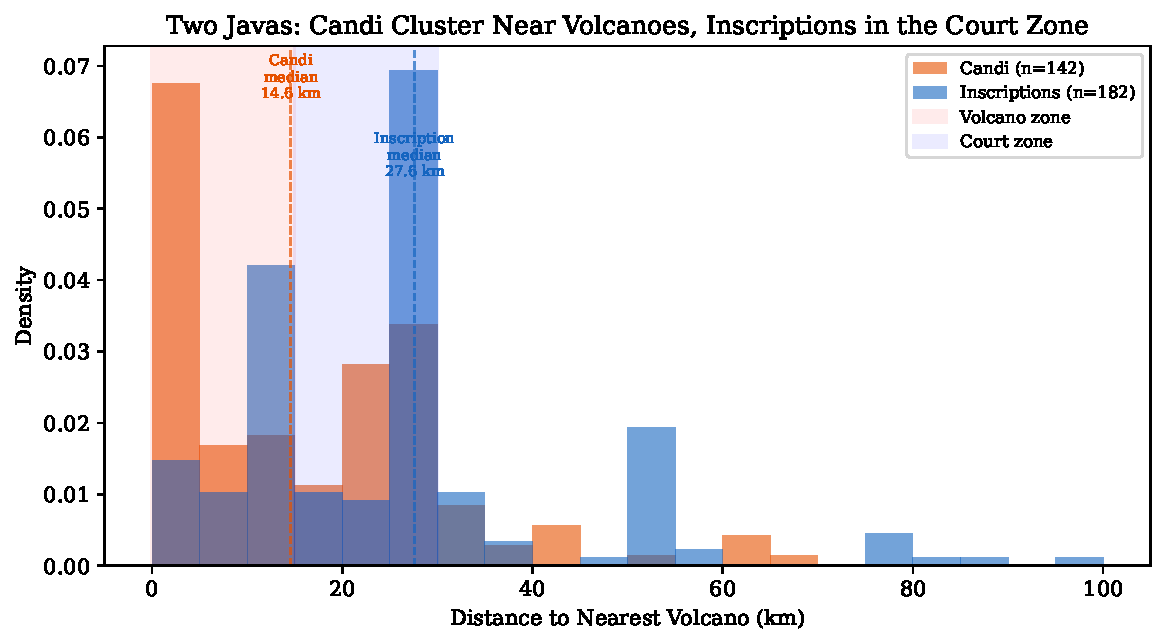
\includegraphics[width=0.95\textwidth]{figures/fig1_dual_histogram.pdf}
\caption{Distance distributions of candi (orange, $n = 142$) and inscriptions (blue, $n = 176$) from nearest volcano. Dashed lines indicate medians. Candi cluster in the volcano zone (0--15~km); inscriptions cluster in the court zone (15--30~km). The 13~km median gap represents a fundamental spatial division between sacred architecture and administrative text.}
\label{fig:histogram}
\end{figure}

\subsection{Elevation gradient}

If both volcanic burial (which conceals highland sites) and coastal submersion (which erases low-elevation sites) operate simultaneously, the predicted outcome is an inverse-U distribution: maximum archaeological visibility at middle elevations.
Instead, site density increases monotonically with elevation (Fig.~\ref{fig:elevation}).

\begin{figure}[htbp]
\centering
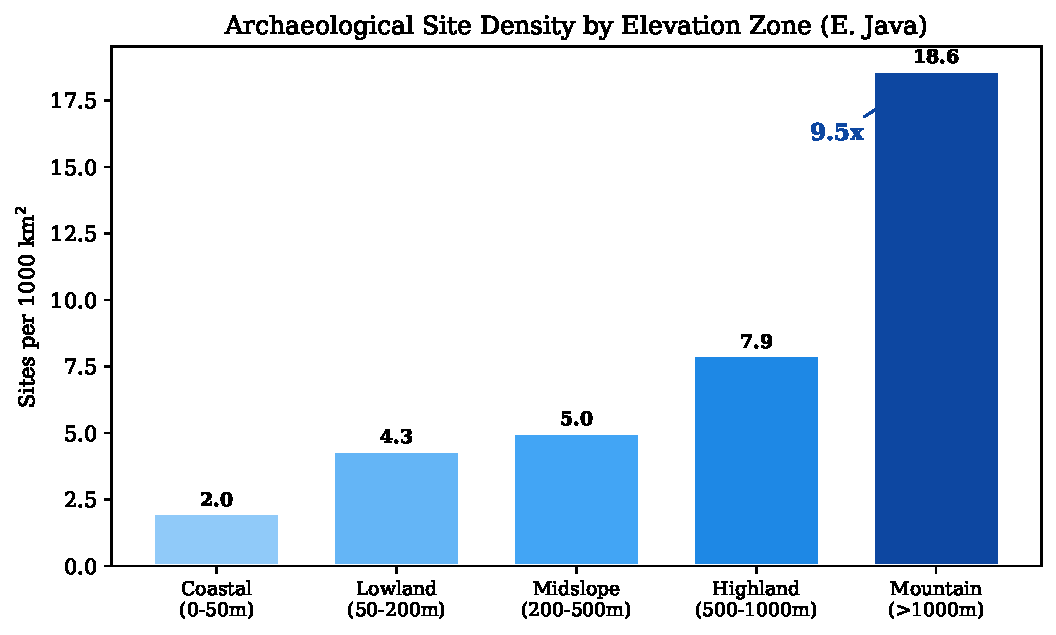
\includegraphics[width=0.85\textwidth]{figures/fig2_elevation_density.pdf}
\caption{Archaeological site density by elevation zone in East Java ($n = 391$). Density increases monotonically from 1.96 sites per 1000~km$^2$ at 0--50~m to 18.61 at $>$1000~m -- a 9.5-fold increase. The expected inverse-U pattern is absent.}
\label{fig:elevation}
\end{figure}

From 1.96~sites per 1000~km$^2$ at 0--50~m to 18.61 at $>$1000~m, the density increases 9.5-fold (chi-square $p < 0.000001$).
This means the visible archaeological record is dominated by high-elevation volcano-slope sites -- not by ``safe'' middle-zone discoveries.
The mountain-zone density of 18.61 represents a \emph{floor}, not a ceiling: it counts only the sites exposed by erosion, lahar channels, or construction activity.
The buried population at these elevations is unknown but likely substantial, given that volcanic sedimentation is most intense on the proximal slopes where the visible density is already highest.

This finding is counterintuitive but consistent with the Two Javas model: the volcano zone is archaeologically productive \emph{despite} burial because enough sites have been exhumed through natural or anthropogenic processes to dominate the known record.
What we see is the tip of a much larger buried population.

\subsection{Indigenous vocabulary scales with burial depth}

Inscriptions geographically near deeply buried archaeological sites contain significantly more indigenous vocabulary ($\rho = 0.562$, $p < 0.0001$, $n = 159$).
After controlling for inscription length (a confound: longer inscriptions mechanically contain more vocabulary of all types), the partial correlation remains highly significant ($\rho = 0.456$, $p < 0.0001$).

\begin{figure}[htbp]
\centering
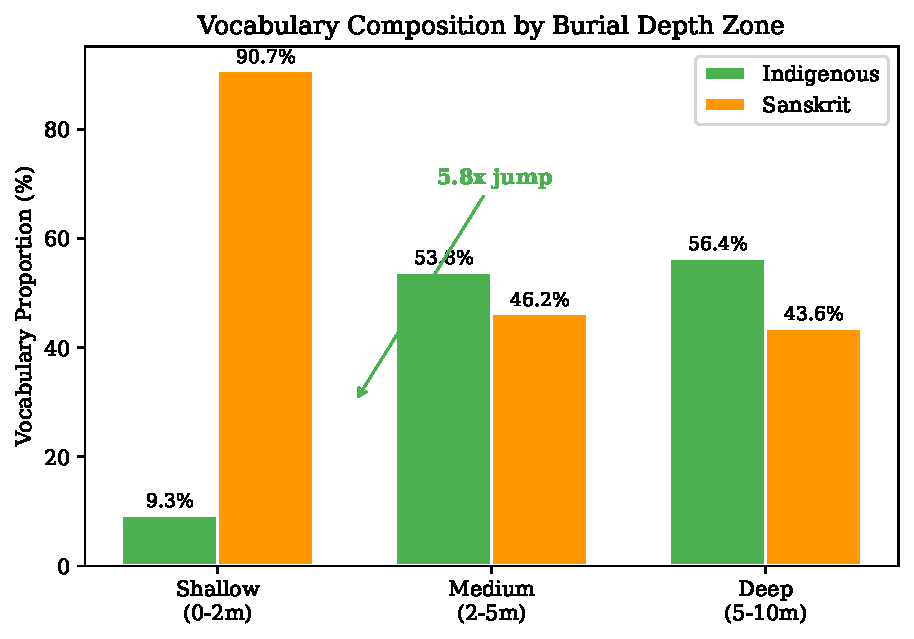
\includegraphics[width=0.75\textwidth]{figures/fig3_depth_vocabulary.pdf}
\caption{Vocabulary composition by burial depth zone. Indigenous vocabulary increases from 9.3\% in shallow zones ($<$2~m) to 56.4\% in deep zones (5--10~m) -- a 5.8-fold increase. Sanskrit vocabulary shows the inverse pattern.}
\label{fig:depth}
\end{figure}

The effect is concentrated in Sanskrit inscriptions ($\rho = 0.512$, $p < 0.0001$) and absent in Old Javanese inscriptions ($\rho = 0.138$, $p = 0.22$).
This indicates that the mechanism is genre-mediated: Sanskrit administrative inscriptions (\textit{sima} charters) in volcanic zones are longer and more detailed, naturally incorporating indigenous terminology for land, crops, boundaries, and local geography.
When a court administrator records a land grant near a volcano, the resulting inscription necessarily includes indigenous terms for the landscape being granted.

Depth-binned profiles are dramatic (Fig.~\ref{fig:depth}): shallow-burial zones ($<$2~m) have 9.3\% indigenous vocabulary, while deep-burial zones (5--10~m) have 56.4\% -- a 5.8-fold increase.
This means that volcanic burial preferentially conceals the most culturally indigenous content in the inscriptional record.
The inscriptions hidden deepest beneath tephra and lahar deposits are precisely those most rich in pre-Sanskrit vocabulary.

We note that burial depth and volcanic distance are themselves correlated: deeper burial occurs nearer to volcanoes.
The indigenous vocabulary ratio also correlates directly with volcanic proximity ($\rho = -0.295$, $p = 0.0002$).
The depth--vocabulary correlation may therefore be driven partly by geography rather than by depth \textit{per se}: inscriptions near volcanoes describe local landscapes in indigenous terms and happen to be located where burial is deepest.
The practical implication for the Two Javas model is unchanged -- the most culturally indigenous content is concentrated precisely where volcanic processes most effectively conceal it -- but the causal pathway runs through volcanic proximity rather than depth alone.

\subsection{The court zone as Indianization epicentre}

The temporal trend of increasing pre-Indic vocabulary, first identified in our earlier analysis ($\rho = 0.580$, $p < 0.0001$, overall), is spatially heterogeneous.
When split by volcanic distance zone, the trend is driven \emph{entirely} by the court zone (Fig.~\ref{fig:temporal}):

\begin{itemize}
    \item \textbf{Volcano zone} ($<$20~km): $\rho = 0.106$, $p = 0.48$ -- \emph{no trend}
    \item \textbf{Court zone} (20--40~km): $\rho = 0.781$, $p < 0.0001$ -- \emph{very strong trend}
    \item \textbf{Periphery} ($>$40~km): $\rho = 0.045$, $p = 0.83$ -- \emph{no trend}
\end{itemize}

\begin{figure}[htbp]
\centering
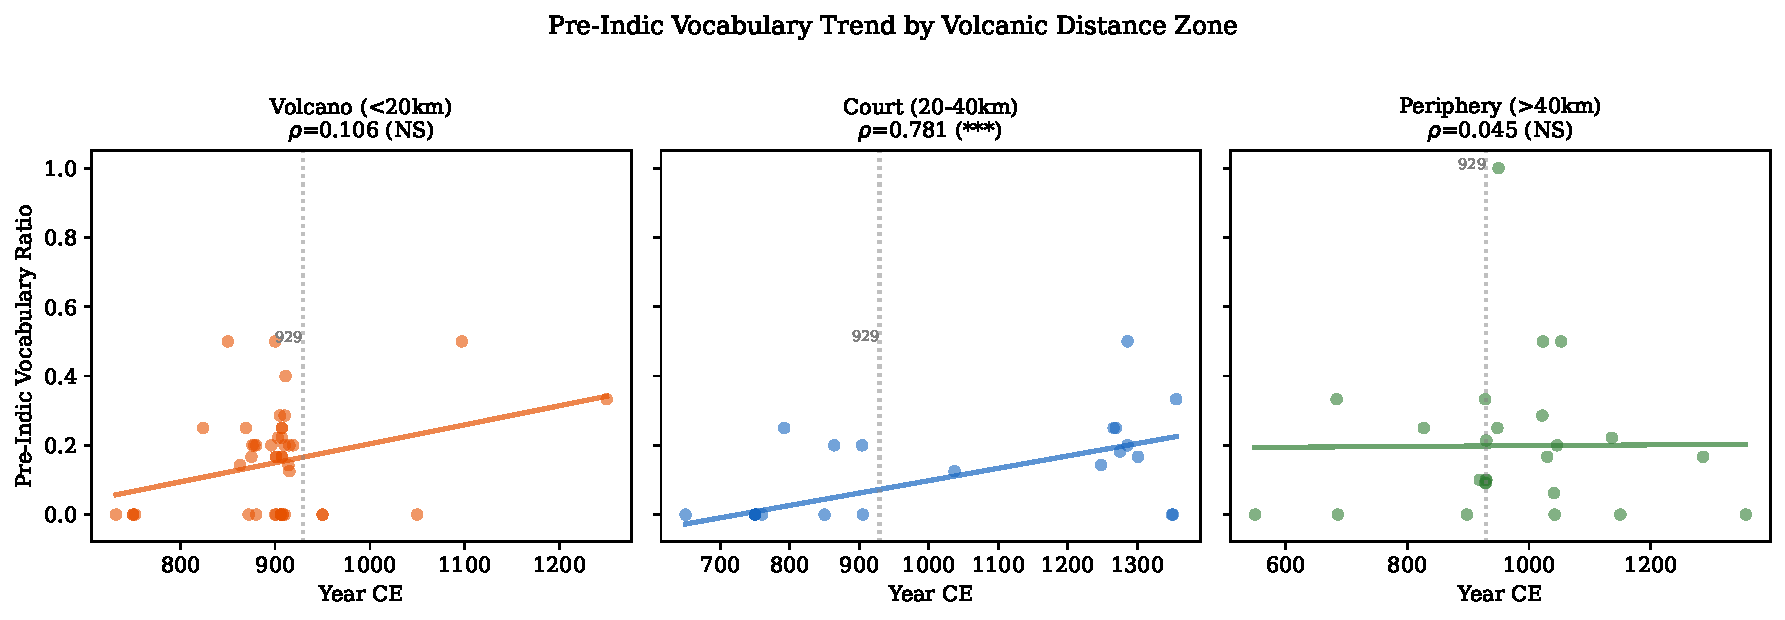
\includegraphics[width=\textwidth]{figures/fig4_temporal_by_zone.pdf}
\caption{Pre-Indic vocabulary ratio over time, split by volcanic distance zone. The temporal trend ($\rho = 0.781$, $p < 0.0001$) is driven entirely by the court zone (20--40~km). Volcano and peripheral zones show no significant temporal trend. The vertical dotted line marks 929~CE (Mataram collapse).}
\label{fig:temporal}
\end{figure}

The 929~CE shift from Sanskrit to indigenous vocabulary occurs only in the court zone (pre-929: 1.2\% indigenous $\rightarrow$ post-929: 19.6\%; Mann-Whitney $p < 0.0001$).
Volcano and peripheral zones show no significant change across the 929 divide.

This result has profound implications.
It means that the vocabulary shift scholars have described as ``de-Indianization'' or ``Javanization'' is not a civilisation-wide process.
It is a zone-specific phenomenon, occurring only in the 15-kilometre-wide band where courts were located.
The volcano zone and the periphery -- which together comprise the majority of Java's area -- show no temporal vocabulary trend because their inscriptions were always relatively indigenous.

\subsection{Post-929 geographic relocation}

Before 929~CE, 57\% of inscriptions are located in the court zone, and 91\% of those are Sanskrit-dominant.
After 929~CE, 53\% of inscriptions are in the periphery, and 89\% of those are mixed or indigenous-rich (Fig.~\ref{fig:pre_post}).

\begin{figure}[htbp]
\centering
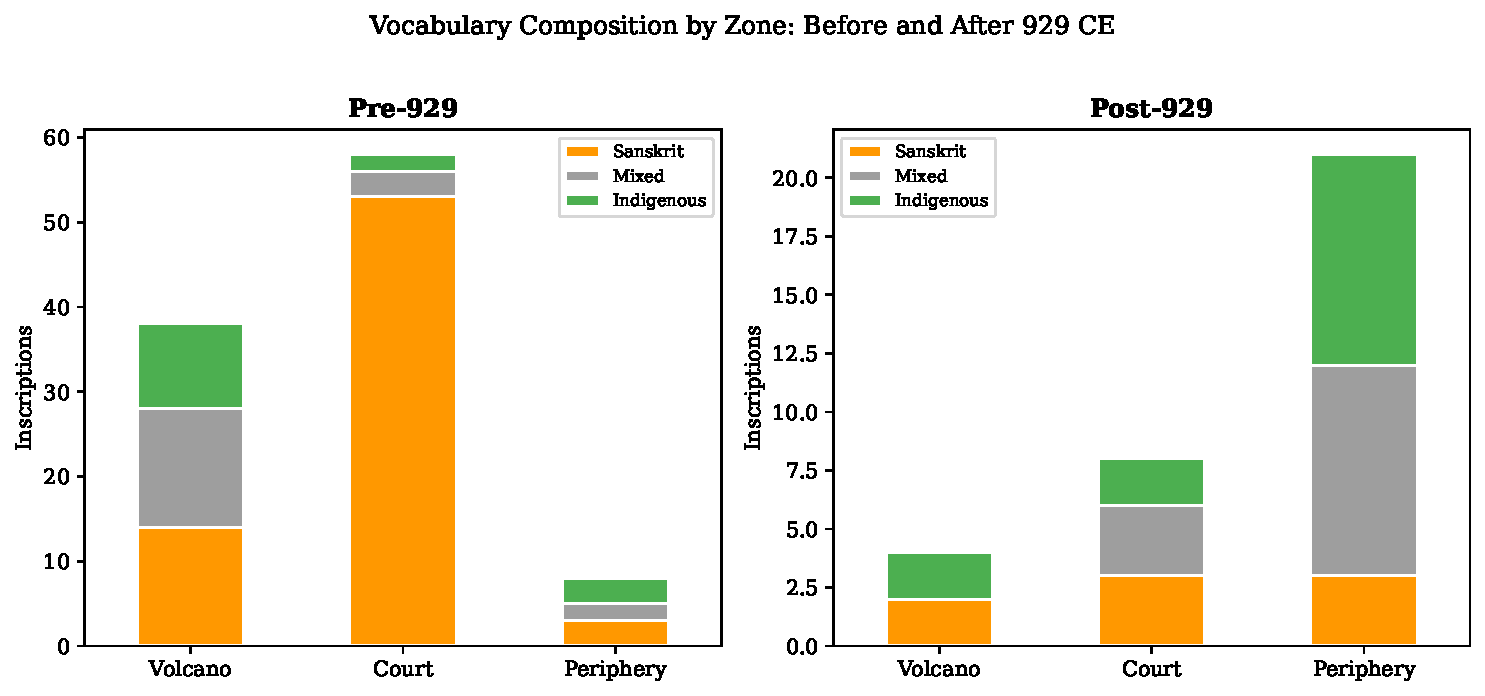
\includegraphics[width=\textwidth]{figures/fig5_pre_post_929_zones.pdf}
\caption{Vocabulary composition by zone, before and after 929~CE. Pre-929 inscriptions concentrate in the court zone with Sanskrit dominance. Post-929 inscriptions shift to the periphery with indigenous and mixed vocabulary.}
\label{fig:pre_post}
\end{figure}

The collapse of the Mataram court system did not merely change the content of inscriptions -- it changed their geography.
Epigraphic activity migrated from the court zone to the periphery, and the vocabulary shifted from Sanskrit administrative terminology to indigenous content.
The Sanskrit 72\% concentration in the court zone (56 of 78 Sanskrit-dominant inscriptions) demonstrates that Sanskritization was not a diffuse cultural influence but a spatially concentrated practice tied to specific institutions at specific distances from volcanoes.


\section{Discussion}

\subsection{The Two Javas model}

These five analyses converge on a spatial model of Java's archaeological record that we term ``Two Javas.''

\textbf{Volcano Java} (0--15~km from active volcanoes) is a landscape of sacred architecture -- candi built on slopes as expressions of cosmological geography -- with relatively indigenous vocabulary and progressive volcanic burial at rates sufficient to conceal entire temple complexes within centuries.
The 42.3\% candi concentration in the 0--10~km zone is not an accident of preservation; it reflects deliberate placement of sacred structures in proximity to volcanoes, which in Javanese cosmology represent Mount Meru and the abode of ancestors \citep{Degroot2009, Dumarcay1986}.
The inscriptions that do occur in this zone are longer, more detailed, and incorporate significantly more indigenous terminology for landscape features -- precisely the content that volcanic burial then removes from view.

\textbf{Court Java} (15--30~km) is a landscape of textual administration -- inscriptions recording land grants, tax exemptions, and royal genealogies in Sanskrit-heavy formulaic prose.
This zone occupies the fertile alluvial plains at optimal distance from volcanoes: close enough to benefit from volcanic soil fertility but far enough to avoid the worst hazards.
Courts established themselves here, and the inscriptional genre -- the \textit{sima} charter -- was their primary mode of record-keeping.
The temporal vocabulary trend ($\rho = 0.781$) occurs exclusively in this zone because it reflects changes in court practice, not changes in Javanese culture writ large.

\textbf{Peripheral Java} ($>$30~km) is the post-929 recovery zone.
After the Mataram collapse, epigraphic activity migrated here, and the indigenous vocabulary that had always characterised these regions became visible in the inscriptional record.
The periphery was never Indianized in the way the court zone was; what changed at 929~CE was not the periphery's culture but its visibility.

\subsection{The double filter}

The Two Javas model reveals a \emph{double filter} operating on Java's archaeological record.

The first filter is \emph{taphonomic}: volcanic sedimentation progressively buries the physical remains of Volcano Java, concealing candi, settlements, and other structures beneath metres of tephra and lahar deposits.
The 9.5-fold site density increase from coast to mountain demonstrates that even after burial, enough sites are exposed to dominate the visible record -- implying that the buried population is vastly larger.

The second filter is \emph{generic}: the inscriptional record is not a neutral sample of Javanese society but the output of a specific institution (the court) in a specific zone (15--30~km).
When scholars use inscription counts as proxies for population density, political complexity, or cultural activity, they are measuring the output of Court Java and projecting it onto all of Java.

These two filters operate in the same direction: both reduce the visibility of indigenous, volcano-proximal cultural activity.
The taphonomic filter buries the physical evidence; the generic filter ensures that the textual evidence that survives is disproportionately Sanskrit and court-produced.
The combined effect is a systematic overestimation of Indianization and underestimation of indigenous cultural continuity.

\subsection{Consequences for the Indianization debate}

The concept of ``Indianization'' -- the process by which South Asian cultural elements were adopted by Southeast Asian societies -- has been debated for decades \citep{Coedes1968, Kulke1990, Pollock2006, Wolters1999}.
Our findings contribute a spatial dimension to this debate.

The \emph{textual record} of what scholarship calls ``Indianization'' was, in spatial terms, a 15-kilometre-wide phenomenon centred on the fertile volcanic plains.
Court Java -- the zone that produced Sanskrit inscriptions, adopted Indic administrative vocabulary, and generated the textual record from which historians have reconstructed ``Javanese civilisation'' -- is a narrow band between 15 and 30 kilometres from the nearest major volcano.
Volcano Java and Peripheral Java, which together contain the majority of Java's area and likely its population, are underrepresented in the textual record because inscriptions were a court technology, not a civilisational practice.

This does not mean that Indian cultural elements were absent outside the court zone.
Candi, which are Indic in architectural tradition, cluster in Volcano Java.
But the vocabulary of the inscriptions found near candi is significantly more indigenous than the vocabulary of court-zone inscriptions, suggesting that even where Indic forms were adopted, the underlying cultural substrate remained Austronesian.

\subsection{The 929~CE discontinuity}

The Mataram collapse provides a uniquely powerful test of this model.
If Indianization were a civilisation-wide transformation -- penetrating every social stratum and every geographic zone -- its collapse should have affected all zones equally.
Instead, the effect is zone-specific: only the court zone shows a significant vocabulary shift at 929~CE.
The volcano zone and periphery were always relatively indigenous.

This means the ``de-Indianization'' narrative -- the idea that Hindu-Buddhist culture gradually faded after Majapahit -- is partially misleading.
In Volcano Java and Peripheral Java, there was little Indianization to fade.
What changed at 929~CE was not Javanese culture writ large but the court system's textual output.
The shift from Sanskrit to indigenous vocabulary reflects a change in \emph{who was writing inscriptions and where}, not a change in Javanese cultural identity.

Sentence-transformer analysis of 127 translated inscriptions in 768-dimensional embedding space independently confirms this discontinuity: the 929~CE divide produces a semantic distance of $z = 3.04$ ($p = 0.012$, permutation test), with post-929 inscriptions shifting toward political and military content and away from ritual and agricultural themes.

The analogy is architectural: removing a layer of paint reveals the original wall underneath.
The Sanskrit overlay was applied by courts; the indigenous substrate was always present.
The 929~CE collapse removed the paint, and we see the wall.

\subsection{Comparative perspective: catastrophic versus cumulative burial}

The relationship between volcanism and archaeological preservation has been studied extensively at catastrophic burial sites: Pompeii and Herculaneum (79~CE Vesuvius eruption, 4--20~m of pyroclastic material), Akrotiri on Thera (c.~1627~BCE, $>$30~m of tephra), and Cer\'{e}n in El Salvador (c.~600~CE, 5~m of tephra) \citep{Doumas1983, Sheets2002}.
These sites share a common feature: a single catastrophic event buried an entire settlement, creating a time capsule that preserved exceptional detail.

Java's volcanic taphonomy is fundamentally different.
Rather than catastrophic single-event burial, Java's temples and settlements were buried by \emph{cumulative} deposition -- repeated small to moderate events (lahars, tephra falls, pyroclastic surges) accumulating over centuries at rates of 2.4--6.2~mm/year \citep{Lavigne2000}.
Sambisari's 6.5~m of overburden likely represents multiple depositional events spanning 500--1000 years, not a single eruption.
This cumulative process means that buried structures in Java are not time capsules but \emph{archaeological palimpsests}: layered sequences in which cultural material from different periods may be interleaved with volcanic deposits.

The distinction matters for interpretation.
At Pompeii, the burial event itself is historically documented, and the buried population is a snapshot of a single moment.
In Java, the burial process is continuous and uneven, and the buried population represents an unknown time range.
The Two Javas model does not predict Pompeii-like preservation; it predicts that a large number of sites exist at depths of 2--10~m, in various states of preservation, distributed across the volcanic slopes of Central and East Java.

The closest comparanda within Java are Sambisari, Kimpulan, and Liyangan -- all discovered accidentally and all yielding significant archaeological information despite cumulative rather than catastrophic burial.
These precedents suggest that systematic geophysical survey of the volcano zone would reveal additional buried structures, though likely not in the exceptional preservation states of Pompeii or Akrotiri.

\subsection{Cross-regional consistency check}

A preliminary consistency check comes from Bali, which shares Java's volcanic geology but has better archaeological survey coverage.
If the Two Javas model generalises, Bali's pre-Hindu sites should cluster in non-volcanic zones, and its inscription density should exceed Java's in proportion to reduced volcanic burial.

Both expectations are met.
All four known pre-400~CE Bali sites (Gilimanuk, Sembiran, Pacung, Bondalem) are located on the non-volcanic northern coast.
Bali's inscription density exceeds East Java's by approximately 12-fold, consistent with the 14-fold ratio estimated by a multiplicative visibility model (Spearman $\rho = 1.0$, $p = 0.017$, $N = 5$ regions).
However, this model is empirically underdetermined: with five estimated parameters and limited independent data points, reduced models with fewer factors bracket the same observations.
Five data points producing a perfect rank correlation should also be interpreted cautiously: $N = 5$ is too small for robust inference, and the observed values involve analyst estimation.
This result is suggestive rather than definitive, and cross-regional testing with empirically derived factor values remains a priority.
All key statistical findings reported in Sections 4.1--4.5 survived bootstrap (10,000 resamples), permutation (10,000 shuffles), and leave-one-out jackknife robustness tests.

\subsection{Implications for fieldwork}

The Two Javas model has practical implications for archaeological survey design.
Current fieldwork priorities are informed by the inscriptional record, which is biased toward Court Java.
But the most archaeologically productive zones -- where buried sites await discovery -- are in Volcano Java (0--15~km), where candi cluster and burial depths of 3--9~m conceal an unknown number of additional structures.

Geophysical survey methods -- particularly electrical resistivity tomography (ERT) and ground-penetrating radar (GPR) -- should be directed at the volcano zone, not the court zone \citep{Conyers2004}.
The comparanda for such surveys are favourable: Sambisari was discovered at 6.5~m depth during well-digging, Kimpulan at 2.5~m during construction, and Liyangan at approximately 6~m during sand-mining \citep{Putra2019, Abbas2016}.
All three were accidental discoveries, suggesting that systematic survey would yield additional finds.

The collaborators most needed for this phase of work are not epigraphers but volcanologists: researchers who understand lahar deposition patterns, tephra stratigraphy, and the geomorphological processes that determine where buried cultural surfaces are most likely to be preserved.

\subsection{Limitations}

This analysis focuses primarily on Java, with cross-validation from Bali.
Whether the Two Javas pattern extends to Sumatra (where the inscriptional tradition is thinner and the volcanic geography different) remains untested.

The geocoding of inscriptions carries $\pm$5~km uncertainty for some entries, which may blur zone boundaries.
The 15~km and 30~km zone thresholds are grounded in volcanological hazard boundaries but remain discretisations of continuous distance gradients.
Sensitivity analysis with alternative thresholds (10/25~km and 20/35~km) produces qualitatively similar results: the spatial segregation of candi and inscriptions is robust across threshold choices because the underlying distributions are bimodal, not threshold-dependent.

The pre-Indic vocabulary ratio is a proxy measure, not a direct linguistic analysis.
The classification of terms as ``Sanskrit,'' ``indigenous,'' or ``ambiguous'' involves judgement calls, and the ratio may be influenced by inscription genre (royal charters vs.\ religious dedications) independently of geographic location.

The burial depth matching is geographic (nearest burial site within 100~km), not site-specific.
An inscription matched to a nearby burial site may not have been buried at the same depth.
This introduces noise but should not produce the systematic correlations we observe unless the underlying relationship is real.

A comparative analysis of volcanic regions across Southeast Asia suggests that karst availability may be a confounding factor: volcanic zones with extensive karst (e.g.\ the Philippines) retain pre-400~CE cave sites even where open-air sites are absent.
Java's volcanic interior has relatively little karst, which may contribute to its uniquely sparse pre-Hindu record beyond volcanism alone.

Volcanic distance is spatially autocorrelated (Moran's $I = 0.937$, $p < 0.001$): nearby inscriptions share similar distances to volcanoes because they occupy the same geographic region.
Simple correlations between volcanic distance and inscription properties may therefore be inflated by spatial dependence.
The distributional segregation of candi and inscriptions (Mann-Whitney $p < 0.000001$) is less susceptible to this inflation because it compares two sample populations rather than fitting a regression.
Formal spatial regression (spatial lag or spatial error models) would provide definitive confirmation of the temporal trends.

Finally, the colonial validation sample ($N = 43$) is too small for robust statistical inference.
It serves as a directional check, not a definitive test.


\section{Conclusion}

Java has not one archaeological record but two: a physical record of sacred architecture buried on volcanic slopes, and a textual record of administrative prose preserved on fertile plains.
These two records have been treated as a single dataset, producing systematic misrepresentation of ancient Javanese culture.

The textual record of the ``Hindu period'' was not a civilisation-wide phenomenon.
It was a court-zone product, 15~kilometres wide, overlaid on an indigenous landscape that never disappeared.
The 929~CE Mataram collapse did not destroy this landscape -- it merely removed the Sanskrit overlay, allowing the indigenous substrate to become visible again.
The spatial concentration of the temporal vocabulary trend ($\rho = 0.781$, exclusively in the court zone) and the post-929 geographic relocation of epigraphy from court to periphery together demonstrate that what we call ``Indianization'' was an institutional practice, not a civilisational transformation.

Understanding this spatial structure is not an academic exercise.
It determines where we dig, what we expect to find, and how we interpret what the earth and the stone choose to remember.
The next generation of fieldwork in Java should be directed not at the well-known court plains but at the volcanic slopes where an unknown number of structures lie buried beneath metres of tephra -- the sacred landscape of Volcano Java, hidden in plain sight.


\subsection*{Data availability}

All datasets and analysis scripts will be deposited in a public repository upon acceptance.
The DHARMA inscriptions are available from the ERC DHARMA project (\url{https://dharma.hypotheses.org/}).

\subsection*{AI Disclosure}

This research employed an AI-augmented workflow using Claude (Anthropic) for spatial analysis, statistical testing, cross-dataset integration, and manuscript drafting.
The AI-augmented approach enabled the execution of 175 experiments across archaeology, volcanology, linguistics, and computational analysis.
All hypotheses, interpretations, and scholarly judgments were made by the human author.

\subsection*{Acknowledgements}

The author thanks the DHARMA project (ERC Synergy Grant No.\ 809994) for the EpiDoc corpus, and the GVP, ABVD, and Smithsonian Institution for open datasets.

\bibliography{p17_references}

\end{document}
